\documentclass[]{article}

% Use utf-8 encoding for foreign characters
\usepackage[utf8]{inputenc}
% For euro symbol
\usepackage{eurosym}
% for http links
\usepackage{hyperref}

% Setup for fullpage use
\usepackage{fullpage}
\usepackage{graphicx}

\usepackage[francais]{babel}

\usepackage{times}
%\usepackage{rotate}
%\usepackage{lscape}

\usepackage{color}
\usepackage{placeins}


\newcommand{\placeholder}[1]{{\noindent \color{red}[ #1 ]}}

%-----Commandes pour page de garde UMons
\usepackage[fs]{umons-coverpage}
\umonsAuthor{François \textsc{Moutier} \href{mailto:francois.moutier0@gmail.com}{francois.moutier0@gmail.com}\\
Alexis \textsc{lecocq} \href{mailto:axtux@hotmail.com}{axtux@hotmail.com}\\
Mehdi \textsc{Maazouz} \href{mailto:souls915@gmail.com}{souls915@gmail.com}\\
Groupe 6}
\umonsTitle{Projet de Génie Logiciel}
\umonsSubtitle{
Activité d'apprantissage S-INFO-015\\
"Lazer Challenge"}
\umonsDocumentType{Rapport de planification\\
19 octobre 2016}
\umonsSupervisor{Sous la direction de  : \\
	Prof. Tom \textsc{mens} (promoteur)} 
% The date (or academic year)
\umonsDate{Année académique 2016-2017}

\begin{document}

%\frontmatter          % for the preliminaries
%\pagestyle{headings}  % switches on printing of running heads
%\mainmatter              % start of the contributions

\umonsCoverPage



%\title{
%{\Huge Rapport de Planification}\\
%Projet de Génie Logiciel\\
%\smallskip
%{\small Activité d'Apprentissage \textsf{S-INFO-015}}\\
%}
%
%\author{Groupe numéro: \textbf{\placeholder{gX}}\\
%Membres du groupe:\\
%\textbf{\placeholder{NOM1 Prenom1} }\\
%\placeholder{continuez avec d'autres noms ici}\\
%}
%
%
%\date{Année Académique \placeholder{20XX-20YY}\\
%\placeholder{Année d'études (par exemple, Bachelier en Sciences Informatiques)}\\
%\vspace{1cm}
%Faculté des Sciences, Université de Mons}






%\title{Projet de Génie Logiciel\\
%Rapport de Planification\\
%Année Académique ****-****\\
%}
%\title{{\Huge Rapport de Planification}\\
%Projet de Génie Logiciel\\
%{\small
%	Unités d'Enseignement \textsf{US-B2-SCINFO-009-M}, \textsf{US-B3-SCMATH-013-M}, \textsf{US-M1-SCINFO-045-M}\\
%	Activité d'Apprentissage \textsf{S-INFO-015}
%}\\
%
%\date{Année Académique 2015-2016\\
%Bachelier en Sciences Informatiques\\
%Bloc complémentaire en Master I Informatique\\
%\vspace{1cm}
%Faculté des Sciences, Université de Mons}
%
%
%%\titlerunning{Rapport de planification -- \textbf{ANNEE ACADEMIQUE}}
%
%
%\authorrunning{Groupe \textbf{**} - \textbf{ANNEE D'ETUDES}} 

%\institute{\textbf{ANNEE D'ETUDES (par exemple BAC 2 INFO ou ANNEE PREPA)}\\
%Faculté des Sciences, Université de Mons\\
%\email{\{ PRENOM1.NOM1 $\mid$ PRENOM2.NOM2 \}@student.umons.ac.be}
%VOUS POUVEZ UTILISER UN AUTRE ADRESSE MAIL QUE CELUI DE L'UMONS SI VOUS LE PREFERIEZ
%}





%\maketitle              % typeset the title of the contribution
%
%\bigskip
%\begin{center} \today \end{center}
%\begin{abstract}
%Ce \emph{rapport de planification} est rendu dans le cadre de l'AA \textsf{S-INFO-015} ``Projet de Génie Logiciel", dispensé par le Prof. \emph{Tom Mens} en année académique \placeholder{****-****}. \placeholder{Le but de ce rapport est de ... COMPLÉTEZ CE RÉSUMÉ.}
%\end{abstract}
%
%\newpage
%%%%%%%%%%%%%%%%%%%%%%%%%%%%%%%%%%%%%%%%%%%%%%%%
%%%%%%%%%%%%%%%%%%%%%%%%%%%%%%%%%%%%%%%%%%%%%%%%




\section{Introduction}\label{sec:intro}

\subsection{Objectifs}

Le travail s'inscrit dans le cadre du cours de Génie Logiciel.
Le travail consiste à réaliser un jeu de type Lazer Challenge regroupant plusieurs variantes et plusieurs niveaux.
Ce dernier a pour but de mettre en avant le travail d'équipe et ainsi, de répartir le travail entre chaque étudiant,
de modéliser un projet et d'en planifier ces différentes étapes.


%%%%%%%%%%%%%%%%%%%%%%%%%%%%%%%%%%%%%%%%%%%%%%%%
\subsection{Exigences fonctionnelles}

Le principe du jeu de base est de lancer des rayons lasers à travers une grille de cases composée de différents types de blocs, chacun 
ayant un comportement spécifique, et d'atteindre une cible placée sur la grille à un endroit précis. Durant les premiers niveaux, le joueur aura 
la possibilité de déplacer ces blocs de manière à atteindre le bloc cible plus facilement. Dans les niveaux plus avancés, les blocs
seront placé en nombres différents ainsi que sur d'autres cases. De plus, le joueur n'aura plus la possibilité de déplacer ces derniers.

Deux modes de jeu seront incorporés, il y aura le mode \textbf{arcade}, où un temps limité obligera le joueur à réussir la partie rapidement.
Et le mode \textbf{practice}, où aucune contrainte de temps ne viendra géner le joueur dans sa partie. Deux options viennent s'ajouter à ces modes, en
effet, le joueur pourra activer l'option \textbf{continuous laser beam}. Dans cette dernière , la source émettra continuellement le rayon laser,
le joueur pourra donc voir directement les effets des blocs sur le rayon quand ce dernier les percutera. L'autre option se nomme \textbf{one-time-only laser beam}
, ici, le joueur devra activer le rayon laser à partir de la source et voir si ce dernier touche la cible du niveau comme prévu. Sinon le jour devra
recommencer la partie.

Trois extensions seront également incluses dans le jeu. La première étant \textbf{level generator}, dont le but est de générer de manière
automatiques des niveaux. La seconde, \textbf{diagonal directions} devra fournir des directions supplémentaires au rayon laser. L'intensité du rayon
laser devra également être prises en compte. Et la dernière, \textbf{saving + multiple users + social network} qui permettra au joueur 
de reprendre la partie exactement à l'endroit où il l'avait quittée. Elle devra également donner la possibilité de créer/se connecter avec un compte
local ou avec un compte facebook et de partager son score sur ce dernier si l'utilisateur le souhaite.

%%%%%%%%%%%%%%%%%%%%%%%%%%%%%%%%%%%%%%%%%%%%%%%%
\subsection{Exigences non-fonctionnelles}

Le jeu doit être stable, pouvoir tourner facilement et ce, même sur des machines plus modestes. Il doit également être modulaire.

%%%%%%%%%%%%%%%%%%%%%%%%%%%%%%%%%%%%%%%%%%%%%%%%
\subsection{Contraintes de temps}

Nous avons quelques contraintes de temps concernant notre projet , les voici :
\\
\begin{itemize}
	\item La date d'échéance pour la remise du rapport de planification est fixée au 19 octobre 2016.
	\item La date d'échéance pour la remise du rapport de modélisation et de la maquette de l'interface utilisateur est fixée au 4 décembre 2016.
	\item La date d'échance pour la remise de l'implémentation concrète du projet est fixée au 31 mars 2017.
	\item Il y a une période de blocus durant les vacances de Noël et il y a une session d'examens qui suit directement cette période.
	\item Maazouz Mehdi et Alexis Lecocq ont des cours du bloc 2 et du bloc 3, ils ont donc des horaires spécifiques, ce qui pourrait ralentir l'avancement du projet.
\end{itemize}


%%%%%%%%%%%%%%%%%%%%%%%%%%%%%%%%%%%%%%%%%%%%%%%%
\subsection{Contraintes de budget}

Nous n'avons aucune contraintes de budget. En effet, le budget alloué pour le projet est de 0 euro. 

\newpage
%%%%%%%%%%%%%%%%%%%%%%%%%%%%%%%%%%%%%%%%%%%%%%%%
%%%%%%%%%%%%%%%%%%%%%%%%%%%%%%%%%%%%%%%%%%%%%%%%
\section{Ressources}\label{sec:organisation}

\subsection{Les ressources humaines (personnel)}
\begin{table}[!htbp]
\begin{center}
\begin{tabular}{p{3cm}|p{1.5cm}|p{2.5cm}|p{5cm}|p{2cm}}
\textbf{NOM Prénom} & \textbf{R\^ole} & \textbf{Durée} & \textbf{Responsabilité(s)} & \textbf{Pourcentage du temps}\\
\hline
MOUTIER Francois & Étudiant & Environ 7 mois & Rapport de planification, de modélisation et implémentation & 32.5\%\\
\hline
LECOCQ Alexis & Étudiant & Environ 7 mois & Rapport de planification, de modélisation et implémentation & 32.5\%\\
\hline
MAAZOUZ Mehdi & Étudiant & Environ 7 mois & Rapport de planification, de modélisation et implémentation & 32.5\%\\
\hline
DUBRULLE Jeremy & Enseignant & Environ 7 mois & Assistance des étudiants dans la réalisation du projet et inspection aux dates clés & 1\%\\
\hline
DEVILLEZ Gauvain & Enseignant & Environ 7 mois & Assistance des étudiants dans la réalisation du projet et inspection aux dates clés & 1\%\\
\hline
MENS Tom & Titulaire & Environ 7 mois & Inspection du projet aux dates clés & 0.5\%\\
\end{tabular}
\end{center}
   \caption{Ressources humaines.}
   \label{tab:RH}
\end{table}

%%%%%%%%%%%%%%%%%%%%%%%%%%%%%%%%%%%%%%%%%%%%%%%%
\subsection{Les ressources logicielles}
GanttProject, logiciel gratuit et open source, sera utilisé pour la réalisation des diagrammes GANTT et PERT.\\
Git, logiciel gratuit et open source, sera utilisé comme gestionnaire de versions sur la plateforme Atlassia Bitbucket (\url{https://bitbucket.org/}, gratuite jusqu'à 5 collaborateurs).\\
Visual Paradigm Standard Edition, gratuit grâce à la licence académique de l’UMons, permettra de réaliser les diagrammes d'utilisation, de classe, de séquence et d'états.\\
\\
Le language de programmation Java 8 sera utilisé pour implémenter le projet.\\
Eclipse et/ou IntelliJ seront utilisé comme environnement de développement.\\
% dernière version 2016-10-17 LibGDX 1.9.4
LibGDX, bibliothèque gratuite et open source, sera utilisée pour son interface graphique, réseau et fichiers ainsi que la gestion de la journalisation.\\
Junit 4.11+, bibliothèque gratuite et open source, sera utilisée pour la réalisation des tests unitaires.\\
% dernière version 2016-10-17 Gradle 3.1
Gradle, logiciel gratuit et open source, sera utilisé pour faciliter le téléchargement des bibliothèques requises, la compilation du code, le lancement des tests unitaires, la génération de la documentation ainsi que la création d'un JAR exécutable.\\
GDX-Facebook 1.2.2 (plugin LibGDX) sera utilisé pour interagir avec l'API facebook.\\
\\
\\
\\
\\
\\
\\
\\
\\

%%%%%%%%%%%%%%%%%%%%%%%%%%%%%%%%%%%%%%%%%%%%%%%%
\subsection{Les ressources matérielles}

\begin{table}[!htbp]
\begin{center}
\begin{tabular}{p{2cm}|p{2cm}|p{1cm}|p{2cm}|p{1.5cm}|p{2cm}|p{2cm}|p{1cm}}
	\textbf{Propriétaire} & \textbf{Nom} & \textbf{Coût} & \textbf{Système d'exploitation} & \textbf{Mémoire vive} & \textbf{Processeur} & \textbf{Carte graphique} & \textbf{Disque}\\
	\hline
	MOUTIER Francois & Tour personnalisée & 1000\euro & Windows 10 64bits & 8Go & Intel Core i5-4690K & Nvidia Geforce GTX-770& SSD 256Go\\
	\hline
	LECOCQ Alexis & Toshiba Satellite S50-B-12R& 800\euro & Ubuntu 16.04 64bits & 16Go & Intel Core i7-4510U & AMD Radeon R7 M260 & SSD 256Go\\
	\hline
	MAAZOUZ Mehdi & Asus S301L & 600\euro & Ubuntu 16.04 64bits et Windows 8 64bits& 6Go & Intel Core i3-4030U & Intel HD Graphics 4400 & SSD 200Go\\
\end{tabular}
\end{center}
\caption{Ressources matérielles.}
\label{tab:RM}
\end{table}

%%%%%%%%%%%%%%%%%%%%%%%%%%%%%%%%%%%%%%%%%%%%%%%%
%%%%%%%%%%%%%%%%%%%%%%%%%%%%%%%%%%%%%%%%%%%%%%%%
\newpage
\section{Analyse des risques}
\subsection{Identification des risques}\label{sec:riskident}

\begin{table}[!htbp]
\begin{center}
\begin{tabular}{|p{3cm}|p{2.5cm}||p{3cm}|p{3cm}|p{2.5cm}|}
\hline
\textbf{Risque} & Catégorie & Probabilité & Sévérité & Importance\\
\hline\hline

\textbf{Délais insuffisant, Dépassement dead-line :} Le projet est rendu après la date limite. &
\textbf{Personnel}&\textbf{Modérée :} Le projet
étant ambitieux et valant un certain nombres de crédits,les membres du groupe sont censés rendre le projet en temps voulu.
& \textbf{Catastrophique :} Le projet sera invalidée et la note obtenue sera de 0 & C'est probablement le risque le plus important à traiter, car 
s'il a lieu, il n'y aura pas de retour en arrière possible et le projet sera invalidé\\
\hline
\textbf{Remise d'un projet incomplet :} Le projet est rendu sans avoir respecté tous les objectifs qui devaient être accomplis 
&\textbf{Produit}&\textbf{Modérée ou Haute :} Le manque de temps, la difficulté des ojectifs à atteindre, l'engagement des membres du groupe peuvent
impacter ce risque &\textbf{Serieuse :} Selon les objectifs qui pourraient ne pas être atteints, la note finale peut grandement varier  & Ce risque possède 
également une imporante capitale, car s'il venait à se produire, la note finale du projet pourrait être insuffisante.\\
\hline
\textbf{Risque personnel :} Un des membres du groupe abandonne le projet  &\textbf{Personnel} &\textbf{Modérée :}
Tous les membres possèdent un PAE différent et vont devoir privilégier certains cours. De plus, 
Un des membres a déjà abandonné le projet de GL deux fois . &\textbf{Serieuse :}Il faudrait alors revoir la
planification pour se répartir le travail. & C'est un risque non négligeable, car la charge de travail pour les membres du groupe restant augmenteraient
de manière significative\\
\hline
\textbf{Perte de données sur BitBucket :} Aucun des membres n'a utilisé BitBucket à ce jour,
ils ne pourront donc pas confirmer la fiabilité des serveurs .&\textbf{Ressources} &\textbf{Faible} En théorie, 
BitBucket étant un outil utlisé à travers le monde et reonnu, ses serveurs devraient être fiables.&\textbf{Sérieuse :} 
La perte du projet sur BitBucket serait grave, mais ce risque peut être géré si les membres du groupe ont une sauvegarde 
local du projet sur leur machine.& Ce risque a une importance mesurable. En effet, sa probabilité
est faible mais il pourrait avoir des conséquences grave ( la perte du projet ) s'il avait lieu et si, il n'avait pas été traité au préalable.\\
\hline
\end{tabular}
\end{center}
   \caption{Analyse des risques génériques, triés par importance.}
   \label{tab:risquesgeneriques}
\end{table}

\begin{table}[!htbp]
\begin{center}
\begin{tabular}{|p{3cm}|p{2.5cm}||p{3cm}|p{3cm}|p{2.5cm}|}
\hline
\textbf{Risque} & Catégorie & Probabilité & Sévérité & Importance\\
\hline\hline
\textbf{Méconnaissance des outils : }Tous les membres du groupe
n'ont jamais utilisés LibGDX et Gradle&\textbf{Personnel}&\textbf{Très Haute : } Le risque est pratiquement inévitable s'il n'est pas
anticipé &\textbf{Serieuse :} L'avancement du projet sera inévitablement impacté par ce risque &Ce risque doit 
absolument être pris en compte par le groupe, de par sa probabilité ainsi que sa sévérité\\
\hline
\textbf{Risque d'incompatibilité :} Un des membres du groupe se trouve sous Windows, les 2 autres membres sont actuellement sous Linux. Il se peut que des problèmes 
interviennent lors des échanges de codes entre les membres du groupe ainsi que dans l'utilisation des outils &\textbf{Ressources} &\textbf{Modérée :} Le langage JAVA est portable même s'il
existe des différences entre les versions Linux et Windows d'un projet &\textbf{Tolérable à catastrophique :}Il se peut que certains bogues apparaissent
sans réellement gêner le projet. Il se peut aussi que le projet ne tourne pas sous Linux, voire Windows .& C'est un risque
très important car il pourrait entraîner la non-validation du projet si ce dernier ne tournait pas correctement sur une des plateformes\\
\hline
\textbf{Manque d'expérience } 2 membres du groupe n'ont à ce jour, réalisé qu'un projet de grande ampleur ( le projet de Ba1), un 
autre membre a réalisé plusieurs projet, mais aucun concernant la conception d'un jeu .
&\textbf{Personnel} &\textbf{Très Haute :}Le manque d'experience impactera forcément le projet.&\textbf{Tolérable : }
Le professeur ainsi que les assistants peuvent aiguiller les élèves dans leurs choix, répondre aux questions éventuelles.& C'est un risque non négligeable, puisque 
qu'il y a une forte probabilité que les élèves y soient confrontés, mais peut facilement être contourné si les élèves osent aller chercher des réponses
aux questions qu'ils se posent au lieu de les laisser en suspens .\\
\hline
\textbf{Mauvaise organisation :} 2 membres du groupes ont des cours du
bloc 2 et 3 et l'autre membre du groupe effectue une année passerelle.&\textbf{Personnel} &\textbf{Haute : }Tous les membres ont un PAE différents.
De plus, les cours du bloc 3 rentrent parfois en conflit avec ceux du bloc 2. &\textbf{Faible :} Même si ce risque venait à se produire, le temps 
alloué à chaque étape du projet est suffisamment long. & C'est un risque qui, probablement, se produira mais à l'importance négligeable. \\
\hline
\end{tabular}
\end{center}
   \caption{Analyse des risques génériques, triés par importance.}
   \label{tab:risquesspecifiques}
\end{table}

%à titre d'information, voici quelques exemples de risques génériques souvent rencontrés dans un projet informatique:
%\begin{itemize}
%\item difficultés techniques imprévues (probl\`eme de versions, probl\`eme de compatibilité, matériel ou logiciel défectueux, perte de données, ...)
%\item difficulté de compréhension (documentation non disponible en fran\c{c}ais, documentation absent, sujet ou domaine complex et difficile à ma\^itriser, ...)
%\item probl\`eme de ressources (matérial non disponible, indisponibilité du directeur ou autres personnes impliquées dans le travail, manque de communication)
%\item probl\`eme d'horaire (manque de temps, horaire de cours inflexible, maladie, ...)
%\item probl\`eme du produit final (incompl\`ete, peu performant, instable, défectueux, manque de documentation, difficile à utiliser ou maintenir, probl\`eme de fiabilité ou sécurité, ...)
%\end{itemize}
%
%Cette liste \textbf{n'est pas exhaustive} et peut varier selon le contexte du travail. Ce qui est important se sont les risques qui sont vraiment spécifiques à votre projet.

%%%%%%%%%%%%%%%%%%%%%%%%%%%%%%%%%%%%%%%%%%%%%%%%
\subsection{Gestion des risques}\label{sec:riskmanagement}
Pour chaque risque, considéré comme important, se situant dans les tableaux de la section 3.1, nous allons expliquer comment :
\begin{enumerate}
\item éviter (ou réduire la probabilité) que le risque se produira
\item vérifier si le risque s'est produit
\item résoudre le risque (si possible) ou réduire l'ampleur et l'impact du risque au moment qu'il se produira
\end{enumerate}

\textbf{Délais insuffisant, Dépassement dead-line  :} \\
1. Etre constamment en contact avec les membres du groupe pour voir l'avancement du projet, revoir la planification de manière régulière
afin de correspondre au mieux aux horaires des membres.\\
2. Revoir la planification régulièrement permettra de voir si les objectifs peuvent être accomplis avant la date limite de ces derniers.\\
3. On ne peut pas réduire l'impact si un ou des objectifs n'ont pas pu être atteints avant la date limite.\\

\textbf{Méconnaissance des outils :}\\
1.  Chercher à se documenter , s'entraîner avec ces outils, aller poser des questions si besoin permettront de réduire le risque lié à la 
méconnaissance des outils.\\
2.  Pour savoir si on a des problèmes avec ces outils , il faut s'exercer avec eux.\\
3.  Il faut prendre l'habitude d'utiliser ces outils le plus rapidement possible, ainsi , le projet ne sera pas retardé ni impacter.\\

\textbf{Remise d'un projet incomplet :}\\
1.  Une bonne gestion du temps, une bonne utlisation des outils ainsi qu'une planification adaptée permettront de réduire le risque d'être incomplet.\\
2.  Les diagrammes GANTT et PERT permettront de voir si les objectifs ont été accomplis en temps voulu.\\
3.  Il faudra revoir la planification ainsi que les diagrammes GANTT et PERT pour limiter l'impact du risque s'il venait à se produire.\\

\textbf{Perte de données sur BitBucket :}\\
1. Celà dépend de la stabilité des serveurs de BitBucket.\\
2. Il suffit d'aller vérifier la page consacrée à notre projet sur leur site.\\
3. Un ou plusieurs membres du groupe devront posséder une copie complète du projet en local, ce qui permettrait 
de résoudre le risque.\\

\textbf{Risque d'incompatibilité :}\\
1. En allant chercher de la documentation concernant les différences qu'ils pourraient y avoir entre l'adaptation du code sur les systèmes d'exploitations
ainsi que dans l'utlisation des outils.\\
2. En compilant et en éxecutant le code sur les différents systèmes d'exploitations.\\
3. On peut résoudre le risque en vérifiant le code et en corrigeant les parties qui ne s'éxecuteraient pas correctement sur un système d'exploitation.

%%%%%%%%%%%%%%%%%%%%%%%%%%%%%%%%%%%%%%%%%%%%%%%%
%%%%%%%%%%%%%%%%%%%%%%%%%%%%%%%%%%%%%%%%%%%%%%%%
\newpage
\section{Répartition du travail}

\subsection{Work Breakdown Structure}

\begin{table}[htbp]
\begin{center}
\begin{tabular}{|p{1cm}|p{5cm}||p{1.5cm}|p{3cm}|p{4cm}|}
\hline
\textbf{ID} & T\^ache & Durée (jours) & Responsable & \% travail\\
\hline\hline
1 & Rapport de la planification & 4 & Tous les étudiants & 33,3\% Moutier, 33,3\% Lecocq, 33,3\% Maazouz\\
\hline
\hline
2 & Conception et Modélisation & 46 & Tous les étudiants & 33,3\% Moutier, 33,3\% Lecocq, 33,3\% Maazouz\\
\hline
2.1 & Rapport de suivi de planification & 46 & Tous les étudiants & 33,3\% Moutier, 33,3\% Lecocq, 33,3\% Maazouz\\
\hline
2.2 & Création des diagrammes & 32 & Tous les étudiants & 33,3\% Moutier, 33,3\% Lecocq, 33,3\% Maazouz\\
\hline
2.3 & Rapport de modélisation & 14 & Tous les étudiants & 33,3\% Moutier, 33,3\% Lecocq, 33,3\% Maazouz\\
\hline
2.4 & Maquette interface utilisateur & 7 & Tous les étudiants & 33,3\% Moutier, 33,3\% Lecocq, 33,3\% Maazouz\\
\hline
\hline
3 & Implémentation & 61 & Tous les étudiants & 33,3\% Moutier, 33,3\% Lecocq, 33,3\% Maazouz\\
\hline
3.1 & Implémentation du jeu de base & 28 & Tous les étudiants & 33,3\% Moutier, 33,3\% Lecocq, 33,3\% Maazouz\\
\hline
3.2 & Implémentation des extensions & 33 & Tous les étudiants & 33,3\% Moutier, 33,3\% Lecocq, 33,3\% Maazouz\\
\hline
3.3 & Phase de testing & 61 & Tous les étudiants & 33,3\% Moutier, 33,3\% Lecocq, 33,3\% Maazouz\\
\hline
3.4 & Rapport d'implémentation & 33 & Tous les étudiants & 33,3\% Moutier, 33,3\% Lecocq, 33,3\% Maazouz\\
\hline
\end{tabular}
\end{center}
   \caption{Tableau des t\^aches.}
   \label{tab:WBS}
\end{table}

%%%%%%%%%%%%%%%%%%%%%%%%%%%%%%%%%%%%%%%%%%%%%%%%
\newpage
\subsection{Etapes clés }

\begin{table}[htbp]
\begin{center}
\begin{tabular}{p{3cm}|p{6cm}|p{6cm}}
	Date & Étape clé & Livrables\\
	\hline
	Mercredi 22 septembre 2016 & Présentation du projet & /\\
	\hline
	Mercredi 28 septembre 2016 & Remise des groupes & Groupes et extensions.\\
	\hline
	Mercredi 19 octobre 2016 & Remise du cahier des charges et du rapport de planification & Cahier des charges et rapport de planification contenant les diagrammes GANTT et PERT.\\
	\hline
	Dimanche 4 décembre 2016 & Remise du rapport de modélisation & Rapport de modélisation et maquette graphique\\
	\hline
	Mercredi 21 décembre 2016 & Réunion d’inspection de modélisation & /\\
	\hline
	Vendredi 31 mars 2017 & Remise de l'implémentation & Implémentation contenant les tests unitaires, la documentation ainsi qu'un exécutable\\
	\hline
	Fin avril ou début mai 2017 & Défense orale du projet & /\\
\end{tabular}
\end{center}
   \caption{Tableau des étapes clés.}
   \label{tab:TEC}
\end{table}

%%%%%%%%%%%%%%%%%%%%%%%%%%%%%%%%%%%%%%%%%%%%%%%%
%%%%%%%%%%%%%%%%%%%%%%%%%%%%%%%%%%%%%%%%%%%%%%%%
\newpage

\section{Ordonnancement}

\subsection{Diagramme GANTT}

%\placeholder{
%Vous devriez inclure et décrire ici un ou plusieurs diagrammes de GANTT correspondant à votre projet, comme par exemple celui montré dans la Figure~\ref{fig:GANTT2}. À vous de choisir comment générer le(s) diagramme(s). Précisez quel outil a été utilisé pour la création de chaque diagramme.
%
%Indiquez, sur le diagramme, les étapes clés et les dépendances entre les t\^aches. Si l'outil que vous avez utilisé ne permet pas de faire cela, vous pouvez mettre cette information dans un tableau séparé, comme par exemple Table~\ref{tab:GANTT}.
%}%end of placeholder

Dans cette section, nous avons construit un premier diagramme de GANTT, généré à l'aide de l'outil GanttProject, nous permettant d'avoir une vue d'ensemble du projet avec ses différentes deadlines et livrables. Celui-ci est repris à la figure ~\ref{fig:GANTT2}:

\begin{figure}[!htb]
\begin{center}
  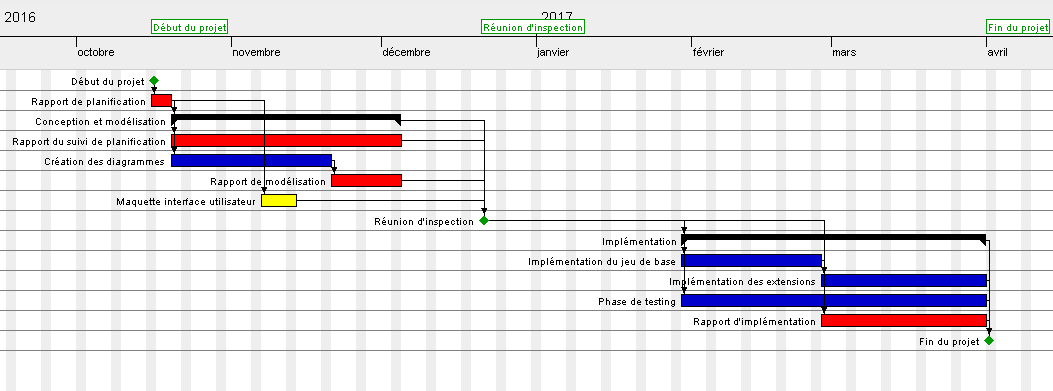
\includegraphics[width=\textwidth]{planif-end.png}
  \caption{Diagramme de GANTT de l'ensemble du projet}\label{fig:GANTT2}
\end{center}
\end{figure}
\FloatBarrier


%\begin{table}[htbp]
%\begin{center}
%\begin{tabular}{|p{2cm}||p{7cm}|p{6cm}|}
%\hline
%\textbf{T\^ache ID } & Nom de la t\^ache & Prédecesseurs \\
%\hline\hline
%\placeholder{id1} & \placeholder{nom1} & \placeholder{liste de prédecesseurs} \\
%\hline
%\placeholder{\ldots} & &  \\
%\hline
%\end{tabular}
%\end{center}
%   \caption{Dépendances entre les t\^aches.}
%   \label{tab:GANTT}
%\end{table}

%%%%%%%%%%%%%%%%%%%%%%%%%%%%%%%%%%%%%%%%%%%%%%%%
\subsection{Diagramme PERT}

%\placeholder{
%Vous devriez inclure et décrire ici un ou plusieurs diagrammes  PERT, comme celui montré dans la figure~\ref{fig:PERT}. À vous de choisir comment générer ce diagramme. Précisez le ou les outils utilisés pour la création de chaque diagramme.
%
%Si l'outil que vous avez utilisé pour générer le diagramme PERT le permet, vous devriez indiquer dans le diagramme, pour chaque t\^ache, la durée, l'effort (en personne/mois), le temps "Earliest Start (ES)", le temps "Latest Start (LS)", le temps l\^ache (\emph{Slack Time (ST)}), et le \emph{Free Float (FF)}. Le diagramme doit également montrer o\`u se trouve le(s) chemin(s) critique(s).
%
%Si l'outil que vous avez utilisé ne le permet pas vous devriez mettre ces informations dans un tableau séparé, comme par exemple la Table~\ref{tab:PERT}.
%}%end of placeholder

Afin de calculer exactement les différentes marges dont nous disposons sur chaque tache ainsi que le chemin critique de notre projet, nous avons construit le diagramme de PERT repris à la figure ~\ref{fig:PERT} \, ainsi que dans le tableau ~\ref{tab:PERT}:

\begin{figure}[!htb]
\begin{center}
  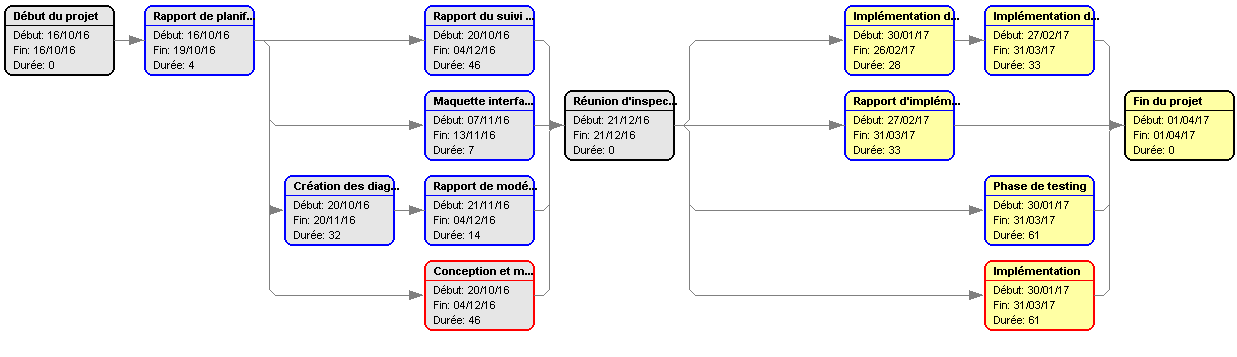
\includegraphics[width=\textwidth]{planif-pert.png}
  \caption{Exemple d'un diagramme PERT.}\label{fig:PERT}
\end{center}
\end{figure}
\FloatBarrier



\begin{table}[htbp]
\begin{center}
\begin{tabular}{|c|p{4cm}||c|p{2cm}|c|c|c|c|c|}
\hline
\textbf{ID} & T\^ache & Durée (j) & Effort (personnes/jour) & ES & LS & ST & FF & T\^ache critique?\\
\hline\hline
%\placeholder{nom ou ID de la t\^ache} & D1 & EFF1 & ES1 & LS1 & ST1 & FF1 & \placeholder{Oui ou non} \\
%\hline
%\placeholder{\ldots} &  &  &  &  &  & & \\
1 & Rapport de la planification & 4 & 2 & 16/10/16 & 16/10/16 & 0 & 0 & oui\\
\hline
\hline
2.1 & Rapport de suivi de planification & 46 & 1/4 & 20/10/16 & 20/10/16 & 0 & 0 & oui\\
\hline
2.2 & Création des diagrammes & 32 & 1 & 20/10/16 & 20/10/16 & 0 & 0 & oui\\
\hline
2.3 & Rapport de modélisation & 14 & 2 & 21/11/16 & 21/11/16 & 0 & 0 & oui\\
\hline
2.4 & Maquette interface utilisateur & 7 & 2 & 07/11/16 & 27/11/16 & 20 & 20 & non\\
\hline
\hline
3.1 & Implémentation du jeu de base & 28 & 2 & 30/01/17 & 30/01/17 & 0 & 0 & oui\\
\hline
3.2 & Implémentation des extensions & 33 & 1 & 27/02/17 & 27/02/17 & 0 & 0 & oui\\
\hline
3.3 & Phase de testing & 61 & 1 & 30/01/17 & 30/01/17 & 0 & 0 & oui\\
\hline
3.4 & Rapport d'implémentation & 33 & 1 & 30/01/17 & 27/02/17 & 28 & 28 & non\\
\hline
\end{tabular}
\end{center}
   \caption{Tableau de PERT}
   \label{tab:PERT}
\end{table}

%%%%%%%%%%%%%%%%%%%%%%%%%%%%%%%%%%%%%%%%%%%%%%%%
\newpage
\subsection{Analyse de l'ordonnancement}

Le chemin critique de notre projet ne prend de sens que si nous prenons en compte le fait que le projet sera en pause durant les mois de décembre et de janvier, dû au fait de la période de blocus et des examens. Les tâches critiques sont dés lors la création des différents diagrammes pour la partie modélisation et l'implémentation du jeu. Ce sont ces tâches qu'il nous faudra contrôler de près tout au long du projet.
%%%%%%%%%%%%%%%%%%%%%%%%%%%%%%%%%%%%%%%%%%%%%%%%
\subsection{Surveillance}

Toutes les semaines, nous mettrons à jour le diagramme de GANTT en y spécifiant l'avancement effectué dans les différentes tâches en cours. Ceci, combiné avec les deadlines et livrables du projet nous permettra de détecter les retards dans le projet. Ces derniers seront comblés en priorité par rapport aux autres tâches.

\end{document}
